\chapter{구현 패턴}
디자인 패턴을 공부하고 나면 어디든 다 쓰고 싶은데, 필요한 지점에 필요한 만큼만 쓰는 것이 좋다.
이 장에서는 디자인 패턴 외에도 복잡한 앱을 개발하는 데 도움이 될 만한 패턴을 이야기 해보자.
%항목에 따라서 동의하기 어려운 게 있다면, 이런 생각이 있다는 정도로 넘어가도 좋겠다.

\section{싱글톤 패턴}
\label{sec:singleton}
% http://www.doubleencore.com/2013/06/context/
% context.tex에 있는 것 제거할 것
안드로이드에서 싱글톤을 잘못 사용하면 메모리 누수 가능성이 많다. 
구조가 복잡한 앱을 보면 속도 이슈 때문에 싱글톤을 많이 사용하는데, 어디선가 메모리 누수가 발생하면 찾을 때 어려움이 많다. 
가급적이면 싱글톤은 꼭 필요한 곳에만 사용하자.\\

싱글톤이라도 Context는 전달해야 유용하게 쓸 수 있는 경우가 많은데, 그럼 Context를 그냥 전달하면 되는가 하면 그렇지 않다.
Context를 그대로 전달하는 경우, 만일 그게 Activity라면 그 인스턴스는 싱글톤에 참조로 남아서 메모리에 계속 남는 문제가 생긴다.
싱글톤을 만들 때 소스 패턴은 아래와 같다. 이것은 support-v4에 포함된 LocalBroadcastManager의 소스이다.
\begin{lstlisting}[frame=single, caption=LocalBroadcastManager.java]
    private final Context mAppContext;
	
    private static final Object mLock = new Object();
    private static LocalBroadcastManager mInstance;

    public static LocalBroadcastManager getInstance(Context context) {
        synchronized (mLock) {
            if (mInstance == null) {
                mInstance = new LocalBroadcastManager(context.getApplicationContext());
            }
            return mInstance;
        }
    }

    private LocalBroadcastManager(Context context) {
        mAppContext = context;
        ...
    }
\end{lstlisting} 
9라인에서 context.getApplicationContext()를 사용함으로써 원래 계속 떠있고 하나뿐인 Application을 Context로 쓰겠다는 의미이다.
많은 안드로이드 책에서도 싱글톤을 만들 때 신경쓰지 않고서 Context를 그대로 전달한 것을 볼 수 있는데 따라하면 안 된다.
특히 SQLiteOpenHelper를 상속한 DB Helper를 싱글톤으로 사용하면서 Context를 그대로 전달한 경우가 많다.\\

% http://stackoverflow.com/questions/3346080/android-references-to-a-context-and-memory-leaks 에도 나옴

이제 조금 더 들어가서 이 내용을 검증하는 방법도 알아보자.
이론적으로 맞는데 정말 그런지 확인할 수 있는 방법이 있을까? 

방법은 3가지가 있는데, 여기서 검증할 내용은 다음과 같다. 
\begin{itemize}
\item 싱글톤에 그대로 넘긴 Activity가 GC가 되지 않는가?
\item getApplicationContext()로 싱글톤에 넘기면 Activity는 적절한 시기에 GC가 이뤄지는가?
\end{itemize}

검증을 위해서 이제 3개의 클래스가 등장한다.\\ 

첫 번째는 싱글톤 클래스이다.
\begin{lstlisting}[frame=single]
public class CalendarManager {

	private static final Object lock = new Object();
	private static CalendarManager instance;
	
	public static CalendarManager getInstance(Context context) {
		synchronized (mLock) {
			if (instance == null) {
				instance = new CalendarManager(context); // (1)
				//instance = new CalendarManager(context.getApplicationContext());
			}
			return instance;
		}
	}
	
	private Context context;
	
	private CalendarManager(Context context) {
		this.context = context;
	}
	
	public String getText() {
		return context.getString(R.string.hello_world);
	}

}
\end{lstlisting}
9라인(1)에서 Context를 직접 전달해서 인스턴스를 생성하였다.\\

두 번째는 싱글톤을 사용하는 Activity이다. AndroidManifest.xml에 android:configsChanges 속성을 따로 넣지 말자.
\begin{lstlisting}[frame=single]
public class CalendarRelatedActivity extends Activity {

	@Override
	protected void onCreate(Bundle savedInstanceState) {
		super.onCreate(savedInstanceState);
		final TextView textView = new TextView(this);
		textView.setText("first run");
		setContentView(textView);
		CalendarManager manager = CalendarManager.getInstance(this); // (1)
	}

	@Override
	protected void onDestroy() {
		android.util.Log.d("suribada", "CalenderRelatedActivity onDestroy");
		super.onDestroy();
	}
	
	@Override
	protected void finalize() throws Throwable { // (2)
		Log.d("suribada", "CalenderRelatedActivity finalize");
		super.finalize();
	}
	
}
\end{lstlisting}
\begin{itemize}
\item 9라인(1)에서 싱글톤 인스턴스를 가져오는데 Activity 자신인 this를 전달하였다.
\item 19라인(2)에서 finalize() 메서드를 오버라이드하고 로그를 남겼다.
\end{itemize}

세 번째는 CalendarRelatedActivity의 Caller이고 메모리 사용량을 계속 키워보면서 테스트하는 Activity이다.
\begin{lstlisting}[frame=single]
public class SingletonTestActivity extends Activity {

    @Override
    protected void onCreate(Bundle savedInstanceState) {
        super.onCreate(savedInstanceState);
        setContentView(R.layout.two_buttons);
    }

    public void onClickButton1(View view) { // (1)
        startActivity(new Intent(this, CalendarRelatedActivity.class));
    }
    
   
	public void onClickButton2(View view) {
		System.gc(); // (2)
	}
	
    private Bitmap bitmap;

    private int width = 480, height = 720;

    public void onClickButton2(View view) { // (3)
        width *= 2;
        bitmap = Bitmap.createBitmap(width, height, Bitmap.Config.ARGB_8888);
    }

}
\end{lstlisting}

첫 번째 검증 방법은 다음과 같다.
\begin{enumerate}
\item CalendarRelatedActivity를 시작한다.
\item 화면 방향을 가로/세로 여러 번 회전한다.
\item Heap 덤프 결과를 확인한다.
\end{enumerate}
s
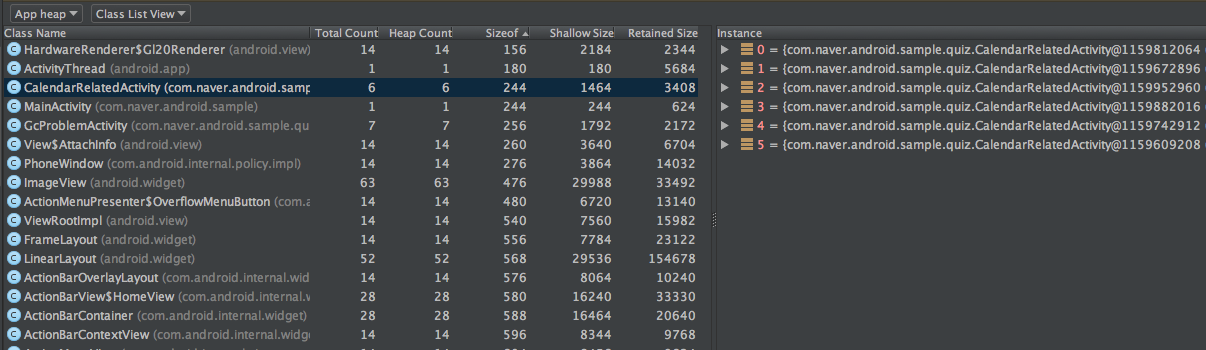
\includegraphics[scale=0.65]{singletonproblem}

\begin{itemize}
\item 9라인(1)에서 CalendarRelatedActivity를 시작한다.
\item 17라인(2)의 메서드에서 클릭할 때마다 createBitmap()에서 width를 2배씩 늘려가면서 메모리 사용량을 키운다.
\end{itemize}

\begin{comment}
검증 방법은 다음과 같다.
\begin{itemize}
\item GC될 때 불리는 finalize() 메서드를 Activity에서 오버라이드하여 Log를 남긴다.
\item 메모리 사용량을 지속적으로 늘려보면서 finalize() 메서드가 불리는 지 확인한다.
\end{itemize}
\end{comment}


이제 테스트 방법은 이렇다.
\begin{enumerate}
\item SingletonTestActivity에서 onClickButton1()을 통해 CalendarRelatedActivity를 실행시킨다.
\item CalendarRelatedActivity에서는 바로 Back 키를 통해서 Activity를 종료시킨다. 이때 onDestory() 메서드가 불린다.
\item SingletonTestActivity에서 onClickButton2()를 여러 번 실행하면서 로그와 메모리 상태를 확인한다.
\end{enumerate}

이제 로그를 살펴보자.
\begin{lstlisting}[frame=single]
09-02 20:46:40.909  20337-20337/com.naver.android.sample D/suribada: CalenderRelatedActivity onDestroy
09-02 20:46:44.079  20337-20337/com.naver.android.sample D/dalvikvm: GC_FOR_ALLOC freed 201K, 31% free 8533K/12332K, paused 8ms, total 12ms
09-02 20:46:44.079  20337-20337/com.naver.android.sample I/dalvikvm-heap: Grow heap (frag case) to 16.449MB for 5529616-byte allocation
09-02 20:46:48.119  20337-20337/com.naver.android.sample D/dalvikvm: GC_FOR_ALLOC freed 2719K, 37% free 11216K/17736K, paused 8ms, total 11ms
09-02 20:46:48.129  20337-20337/com.naver.android.sample I/dalvikvm-heap: Grow heap (frag case) to 24.342MB for 11059216-byte allocation
....
09-02 20:46:59.589  20337-20337/com.naver.android.sample D/dalvikvm: GC_FOR_ALLOC freed 43201K, 49% free 92216K/179752K, paused 13ms, total 14ms
09-02 20:46:59.589  20337-20337/com.naver.android.sample I/dalvikvm-heap: Forcing collection of SoftReferences for 176947216-byte allocation
09-02 20:46:59.609  20337-20337/com.naver.android.sample D/dalvikvm: GC_BEFORE_OOM freed 9K, 49% free 92206K/179752K, paused 15ms, total 15ms
09-02 20:46:59.609  20337-20337/com.naver.android.sample E/dalvikvm-heap: Out of memory on a 176947216-byte allocation.
\end{lstlisting}

계속 메모리 사용량이 늘어가면서 마지막 라인에서 OOM이 발생했는데, 여기서 포인트는 OOM이 발생했다는 것이 아니다.
OOM이 될 때까지도 CalenderRelatedActivity의 finalize()가 불리지 않았다.
즉 CalenderRelatedActivity는 GC 대상이 끝까지 아니었다는 것이다.\\

이제 CalendarManager에서 주석으로 있던 부분으로 대체해서 테스트해보자.
즉 context를 직접 쓰지 않고 context.getApplicationContext()를 전달한 것이다.
\begin{lstlisting}[frame=single]
09-02 20:51:27.099  25785-25785/com.naver.android.sample D/suribada: CalenderRelatedActivity onDestroy
09-02 20:51:29.739  25785-25785/com.naver.android.sample D/dalvikvm: GC_FOR_ALLOC freed 199K, 31% free 8532K/12332K, paused 15ms, total 19ms
09-02 20:51:29.739  25785-25785/com.naver.android.sample I/dalvikvm-heap: Grow heap (frag case) to 16.448MB for 5529616-byte allocation
09-02 20:51:29.749  25785-25794/com.naver.android.sample D/suribada: CalenderRelatedActivity finalize // (1)
09-02 20:51:30.399  25785-25785/com.naver.android.sample D/dalvikvm: GC_FOR_ALLOC freed 2719K, 37% free 11214K/17736K, paused 12ms, total 12ms
...
09-02 20:51:36.829  25785-25785/com.naver.android.sample E/dalvikvm-heap: Out of memory on a 176947216-byte allocation.
\end{lstlisting}
4라인(1)에 바로 CalenderRelatedActivity의 finalize()가 불리었으니, GC가 정상적으로 된 것을 알 수 있다.

\section{마커 인터페이스}
마커 인터페이스는 Effective Java Item 37에 내용이 있고, \url{http://blog.doortts.com/153}에도 간략히 나온다.
마커 인터페이스의 기본 내용은 메서드 선언이 비어 있는 인터페이스라는 것이다.
Serializable도 그 예인데, 말 그대로 표식(marking) 용도로 인터페이스를 사용한다.\\

복잡한 부분은 클래스 구성을 잘 하면 쉽게 해결되는 부분이 많다.
쇼핑 앱을 예로 들어보자. 상품에는 여러 카테고리가 있어서, 구매가 이뤄지면 카테고리별로 백그라운드에서 하는 일이 다르다.
\begin{itemize}
\item A/B 카테고리는 구매패턴 분석을 위해 통계 DB에 데이터를 넣는다(someOperationW).
\item A/C/E 카테고리는 문자로 상품제공자에게 알리고(someOperationX), C/D/E 카테고리는 메일로 알린다(SomeOperationY).
\item B/D/E 카테고리는 사용자에게 다시 알림을 보낸다(someOperationZ).
\end{itemize}

이 로직을 구현하는 기본적인 방법은 아래와 같다.
\begin{lstlisting}[frame=single]
	if (A || B) { 
		someOperationW(); 
	}
	...
	if (A || C || E) { 
		someOperationX(); 
	}
	..
	if (C || D || E) { 
		someOperationY(); 
	} 
	..
	if (B || D || E) { 
		someOperationZ(); 
	}
	..
\end{lstlisting}
처음에는 이 방법도 쓸만한 것 같다.
그런데 어느 날 카테고리가 추가되고 Operation도 여러 개 더해진다면 주의를 기울여야 한다.
만일 평소에 작업하던 개발자가 자리라도 비운다면 긴장도가 높아질 것이다. 
이 복잡도를 해결하는 시도는 아래처럼 할 수 있다.
\begin{itemize}
\item 상위 클래스에는 someOperationXxx() 메서드를 모두 구현한다.
\item 각 카테고리를 나타내는 하위 클래스를 만들어서 someOperationXxx()를 순차적으로 호출하거나, 필요한 경우 오버라이드한다(오버라이드 필요성은 있다. 메일을 보낼때 특정 문구가 필요한 경우가 그런 예일 것이다).
\end{itemize}

이렇게 하면 해당 카테고리의 정책에 집중할 수 있어서 상황은 나아지지만 남은 문제점도 있다.
\begin{itemize}
\item 작업은 순서가 중요한 경우가 많다. 해당 카테고리의 특정 API를 네트워크 호출하고, 그 결과를 DB에 저장하는 경우를 예로 들 수 있다.
하위 클래스에서 상위 클래스의 메서드를 여러 개 호출하는 식이면, 순서를 잘못 호출할 가능성이 생긴다.
\item 카테고리가 추가될 때 기존 카테고리와 유사한 부분이 많다면, 이를 또 상속받고 싶은 유혹이 생긴다.
카테고리끼리의 상속은 정책이 바뀐다면 뜯어고칠 부분이 많아진다.
\end{itemize}

두 가지 중에서 첫 번째 내용이 더 중요하다. 
클래스 상속을 피할 수는 없지만, 상위 클래스에서는 작업 순서까지 지정하고 상속 단계를 최소한으로 할 수 있는 방법을 찾는 게 좋다.\\

여기에서 필자가 선택한 방법이 마커 인터페이스이다. 
현재 처한 상황에서 마커 인터페이스를 적용하는 방법을 보자.
이제 각 작업을 마커 인터페이스로 만든다.\\

\begin{lstlisting}[frame=single]
public interface Markable1 { }

public interface Markable2 { }

public interface Markable3 { }

public interface Markable4 { }
\end{lstlisting}

 
이제 각 카테고리별로 하위 클래스를 만든다.

\begin{lstlisting}[frame=single]
Aclass extends Category implemtens Markable1, Markable2 { }

Bclass extends Category implements Markable1, Markable4 { }

Cclass extends Category implements Markable2, Markable3 { }

Dclass extends Category implements Markable3, Markable4 { }

Eclass extends Category implements Markable2, Markable3, Markable4 { }
\end{lstlisting}

 
상위 클래스에서는 인스턴스를 체크해서 해당 작업을 진행한다.
\begin{lstlisting}[frame=single]
	if (this instanceof Markable1) { 
		someOperationW();
	}
 	...
	if (this instanceof Markable2) { 
		someOperationX();
	}
	..
	if (this instanceof Markable3) { 
		someOperationY(); 
	} 
	..
	if (this instanceof Markable4) { 
		someOperationZ();
	}
	..
\end{lstlisting}
이렇게 하면 상위 클래스에서 각 Operation 순서가 정해지고, 
각 카테고리의 정책이 바뀌면 카테고리 클래스에서 implements하는 것만 조정하면 된다.
작업이 추가되면 MarkableN 인터페이스를 하나 더 만들고서 규칙에 맞추기만 하면 된다.\\

마커 인터페이스는 파라미터가 많은 메서드를 호출할 때도 도움이 된다.
아래와 같은 메서드 시그너처가 있다고 하자.
\begin{lstlisting}[frame=single]
	public static void showPhoneDialog(Context context, String phoneNumber, String keyword, boolean isNaverUser, boolean isKorean) {
		...
	}
\end{lstlisting}

안드로이드 프레임워크 소스에도, 전달되는 파라미터가 많은 메서드를 흔하게 볼 수 있다. ActivityThread의 bindApplication() 메서드는 파라미터가 18개나 된다.
파라미터가 많다면 파라미터에 따른 조건문도 복잡해진다.
이렇게 파라미터가 많은 메서드에서, 동일한 타입이 연달아 나오는 경우 실수할 가능성이 많다. 
showPhoneDialog() 메서드에서 phoneNumber와 keyword, 그리고 isNaverUser와 isKorean은 타입이 동일하기 때문에 호출하는 쪽에서 데이터를 반대로 넣을 수 있다.
타입은 맞기 때문에 컴파일러에서는 검증할 게 없고, 결국 사람이 제대로 값을 써주어야 한다.
Builder 패턴을 통해 파라미터 갯수를 줄이려는 노력을 할 수도 있다. 그래도 아직은 파라미터가 아주 많지는 않으니까(5개 이내) 파라미터를 더 늘리지 않는 쪽에 주의해보자.\\

앱에 새로운 기능을 추가하면서 여러 화면이 생겼고, 여기서도 showPhoneDialog() 메서드를 호출하였다.
그런데 이 기능에서는 showPhoneDialog()에서 하는 여러 작업 가운데 한 가지는 필요 없다는 얘기가 들려왔다.  내부에서 savePhoneState() 메서드를 호출하는데, 이 기능에서만은 savePhoneState() 메서드 호출이 불필요하다는 것이다.
이때 고민이 된다. boolean 파라미터를 하나 추가하고서 이것으로 체크할까? 그러면 파라미터에 boolean이 3개 연속이 되어서 호출하는 쪽에서 더 혼동이 생길 것이다.
\begin{lstlisting}[frame=single]
	public static void showPhoneDialog(Context context, String phoneNumber, String keyword, boolean isNaverUser, boolean isKorean) {
		showPhoneDialog(context, phoneNumber, keyword, isNaverUser, isKorean, false);
	}

	public static void showPhoneDialog(Context context, String phoneNumber, String keyword, boolean isNaverUser, boolean isKorean, boolean ignorePhoneState) {
		...
		if (!ignorePhoneState) {
			savePhoneState();
		}
		...
	}
\end{lstlisting}

다른 쪽 호출 로직에 덜 영향을 주기 위해 5라인에서 메서드를 오버로드했지만, 두 번째 메서드도 결국 public 메서드이기 때문에 역시 파라미터가 많은 문제점을 안고 있다.\\ 

이때 쓸 수 있는 방법도 바로 마커 인터페이스다. Context 파라미터에 컴포넌트 this가 주로 전달되는데, 컴포넌트에 마커 인터페이스를 하나 연결해주면 된다.

\begin{lstlisting}[frame=single]
public TaxiActivity extends Activity implements IgnorePhoneState {
	...
}
\end{lstlisting}

\begin{lstlisting}[frame=single]
	public static void showPhoneDialog(Context context, String phoneNumber, String keyword, boolean isNaverUser, boolean isKorean) {
		...
		if (!context instanceof IgnorePhoneState) {
			savePhoneState();
		}
		...
	}
\end{lstlisting}	
	
마커 인터페이스는 마커 애노테이션(Marker Annotation)으로 대체 가능한 것을 알 수 있다.

\begin{lstlisting}[frame=single]
@Retention(RetentionPolicy.RUNTIME)
@interface Markable1 {
}

@Retention(RetentionPolicy.RUNTIME)
@interface Markable2 {
}

@Retention(RetentionPolicy.RUNTIME)
@interface Markable3 {
}

@Retention(RetentionPolicy.RUNTIME)
@interface Markable4 {
}
\end{lstlisting}

\begin{lstlisting}[frame=single]
	Class clazz = this.getClass();
	if (clazz.isAnnotationPresent(Markable1.class)) {
		someOperationW();	
	}
 	...
	if (clazz.isAnnotationPresent(Markable2.class)) {
		 someOperationX();
	}
	..
	if (clazz.isAnnotationPresent(Markable3.class)) {
		someOperationY();
	} 
	..
	if (clazz.isAnnotationPresent(Markable4.class)) {
		 someOperationZ();
	}
	..
\end{lstlisting}

이런 경우에는 인터페이스나 애노테이션을 쓰는 게 별 차이가 있어 보이지 않는다. 다만 인터페이스를 구현하면 하위 클래스에도 영향이 있지만, 애노테이션을 쓰는 경우 상속과 관련없이 각 클래스마다 개별적으로 애노테이션을 지정해야 한다. 어느 것이 맞는 게 아니라 방식을 이해하고 선택하도록 하자.

\section{Fragment 정적 생성}
아래 두 가지 패턴 가운데 첫 번째 패턴이 개발자 사이트나 많은 샘플에서 주로 쓰고 있다. 그런데 왜인지는 잘 나와있지 않다.
\begin{lstlisting}[frame=single]
   public static ContentFragment newInstance(int left, int right) {
        ContentFragment fragment = new ContentFragment();

        Bundle args = new Bundle();
        args.putInt(LEFT, left);
        args.putInt(RIGHT, right);
        fragment.setArguments(args);

        return fragment;
    }

    @Override
    public View onCreateView(LayoutInflater inflater, ViewGroup container, Bundle savedInstanceState) {
        View view = inflater.inflate(R.layout.content_result, container, false);
        TextView result = (TextView) view.findViewById(R.id.result);
        int sum = getArguments().getInt(LEFT) + getArguments().getInt(RIGHT);
        result.setText("결과=" + sum);
        return view;
    }
\end{lstlisting}

\begin{lstlisting}[frame=single]
    private int left;
    private int right;

    public void set(int left, int right) {
        this.left = left;
        this.right = right;
    }

    @Override
    public View onCreateView(LayoutInflater inflater, ViewGroup container, Bundle savedInstanceState) {
        View view = inflater.inflate(R.layout.content_result, container, false);
        TextView result = (TextView) view.findViewById(R.id.result);
        int sum = left + right;
        result.setText("결과=" + sum);
        return view;
    }
\end{lstlisting}

첫 번째 방식은 사용하려는 변수를 어렵게 넣고 빼는 거 같은데, 사용하기에는 두 번째가 편한 것 같다.
그래서 두 번째 방식을 선택하려는 유혹이 있는데, 첫 번째 방식을 권장하는 이유는 바로 Configuration 변경과 Activty의 예기치 않은 종료에 대응할 수 있기 때문이다. 첫 번째 방식은 값을 유지하고 두 번째는 값을 유지하지 못한다.\\

프레임워크 소스를 통해서 원인을 파악해보자.
\begin{itemize}
\item Fragment에는 FragmentState라는 Parcelable한 내부 클래스가 있고 여기에 Fragment의 setArguments() 메서드에 전달한 Arguments Bundle을 저장한다.
\item Activity의 onSaveInstanceState()에서 FragmentManagerImpl의 saveAllState()를 호출해서 FragmentState 값들을 저장한다.
\item FragmentState에 속한 것이 아닌, 두 번째 방식처럼 우리가 만든 Fragment의 변수들은 당연히 저장이 안 된다.
\end{itemize}

두 번째 방법에서도 값을 유지할 수는 있는데, 바로 
Fragment에서 onSaveInstanceState()를 오버라이드하는 것이다.
\begin{lstlisting}[frame=single]
    @Override
    public View onCreateView(LayoutInflater inflater, ViewGroup container, Bundle savedInstanceState) {
        View view = inflater.inflate(R.layout.content_result, container, false);
        TextView result = (TextView) view.findViewById(R.id.result);
        if (savedInstanceState != null) {
            left = savedInstanceState.getInt(LEFT);
            right = savedInstanceState.getInt(RIGHT);
        }
        int sum = left + right;
        result.setText("결과=" + sum);
        return view;
    }

    @Override
    public void onSaveInstanceState(Bundle outState) {
        outState.putInt(LEFT, left);
        outState.putInt(RIGHT, right);
        super.onSaveInstanceState(outState);
    }
```
\end{lstlisting}
이렇게 하는 것보다는 Fragment 정적 생성이 더 단순하다. 프레임워크에서 이미 제공하는 기능을 피할 이유는 없다.

\begin{comment}
\subsubsection{하위 클래스에서 boolean 리턴 메서드 오버라이드}
boolean을 리턴하는 메서드를 쓰는 것도 비슷하긴 하다.
 
상위 클래스에서 아래와 같이 사용한다.
	
\begin{lstlisting}[frame=single] 
	public void execute() {
		if (isAttribute1()) {
 			someOperationW();
		}
		...
	}
 
	protected boolean isAttribute1() {
		return false;
	}
\end{lstlisting}
 
하위 클래스에서 isAttributeA() 메서드를 필요할 때 오버라이드 하는 방식이다.
나도 이 방법을 쓰는 경우가 있긴 한데, marker interface는 좀 더 복잡한 케이스에 더 맞는다.\\

경우를 좀 생각해보자.
해야 할 if  문이 10개라고 하면 10개의 boolean을 리턴하는 메서드가 필요해진다.
하위 클래스에서는 어느 것에 true이고, 어느 것에 false인지를 정해주면 되는데, 갯수가 많아지면, 나중에 정책이 바뀔 때 작업에서 혼돈이 있지 않을까.\\
 
한 가지 비유를 생각해보았다.
10권의 지정된 책이 있다. 내가 속한 조직의 구성원들한테, 각 책을 갖고 있는지 여부에 따라서 뭔가를 해주고 싶다. 책을 사준다든가, 교육을 보내준다든가 하는 게 있을 것이다.\\
 
이때 각각의 boolean 리턴 메서드를 만들 수 있다. hasEffectiveJava(), hasAndroidHacks(), ...
각 구성원 클래스는 이것을 오버라이드 해서 갖고 있는 책에다 true를 리턴하게 하면 된다.\\

그런데 어느날 책 장터가 열려서 각자 갖고 있는 책들이 다 바뀌어 버렸다.
이때 또 각각 찾아서 true/false를 바꿔주면 된다.\\
 
그런데 이런 경우에 이게 더 쉽지 않을까? 책1 가지고 있는지, 책2 가지고 있는지 계속 묻는 거 보다, 자기가 갖고 있는 책만 나열하라고 하는 것이다.
boolean 메서드를 쓰는 방식이 책 각각에 대해서 묻는 것이고, marker interface를 쓰는 건 갖고 있는 것만 나열하는 방식이다.\\
 
한두개라면  boolean 메서드 방식이 확실히 더 낫겠지만, 갯수가 막 늘어나면 한계가 보인다는 것이다.
결국 100\% 정답은 없고, 저울질을 해봐야 한다.\\
 
marker interface의 장점이 또 하나 있다. 
10권에서 한권이 늘어나도, 수정이 간단하다. 인터페이스 하나 만들고, 각 하위 클래스에다 implements 에 인터페이스 추가만 하면 된다.
아무리 IDE가 편리해 졌다지만, 메서드 생성하고 true/false 리턴하는 번거로움 보다 낫다.\\

\subsubsection{EnumSet 또는 bit flag 사용}
오버라이딩할 필요가 있는데 속성의 수도 많아 메서드를 수십 개 만들어야 하는 상황이라면 EnumSet을 활용할 수도 있다.

\begin{lstlisting}[frame=single]  
    @Override 
    protected EnumSet<Attr> getAttributes() { 
        return EnumSet.of(Attr.A, Attr.B, Attr.D);
    }

\end{lstlisting}

상위 클래스에서 다음과 같이 쓴다. 
\begin{lstlisting}[frame=single] 
	EnumSet<Attr> enumSet = getAttributes();
  	if (enumSet.contains(Attr.A)) { 
  		someOperationW();
  	} 
\end{lstlisting}
 
EnumSet과 유사한 방식으로 bit field를 사용할 수도 있다. Effective Java Item 32에는 bit field 보다는 EnumSet을 쓰라고 나오지만, bit field도 안드로이드에서 많이 쓰이는 방식이다.\footnote{안드로이드에서는 퍼포먼스 이슈 때문에 Enum보다는 int 상수를 쓰라는 가이드가 아직 남아있다. Effective Java와 상충되는 여러 가지 가이드가 있지만, 갈수록 고려할 내용에서 줄어들고 있다.}
\end{comment}

\begin{comment}
\subsubsection{Model View Presenter 패턴}
전체적으로 쓰기에는 무리가 있다.
뷰 네비게이션 정도로만 사용하는 것이 좋지 않을까.
Presenter를 쓰면 뷰를 다른 뷰로 교체하는 게 수월한 부분은 큰 이익입니다.
여러 개의 뷰를 하나의 Presenter로 커버하는 건 간단치는 않은 듯 하고요. 
"리스트뷰가 그리드뷰로 바뀌었다" 이 정도의 요구사항이면 그럴 수 있지만, 실제 요구사항은 정말 복잡다단하잖아요.
 
Presenter에서 네트웍 상태를 체크해서 뷰에 반영하기 위해서는 어찌해야 될까 생각해봤습니다.
Context 가 Presenter에 전달되어 있어야 겠죠. Context가 전달되어야만 할 수 있는 게 무지 많습니다.
 
Context만 전달되면 모든게 다 될까요? 경우에 따라서는 액티비티가 전달이 되어야 할 수도 있습니다. 
그렇다면 액티비티에서는 바로 XXX 메서드호출해서 체크하는 것을 Presenter에서는  ((Activity) context).XXX 해야하는 경우까지 생길 수 있겠죠.
 
요지는 뭔가 하면 디펜던시를 어떻게 완전히 끊느냐입니다.
 
웹에서 유명한 프레임웍이 스트러츠와 스프링이 있습니다.
초기에 스트러츠에서는 액션을 만들때 HttpServletRequest라는 걸 계속 전달을 해왔습니다. 근데 이 Servlet API 종속때문에 테스트도 어렵고, 그 자체로 완결성을 갖기가 어려웠어요.
그런데 스프링에서는 프레임웍 내부에서 알아서 다 하고, 개발자가 POJO 만 만들면 되었어요.
POJO만 만들었으니, 이건 꼭 웹에서만 사용하는 것도 아니고, 일반 애플리케이션에서도 사용하는 데 아무 문제가 없었죠.
 
안드로이드 MVP 패턴을 전적으로 사용함에도 코드 복잡성을 줄이기 위해서는 일종의 프레임웍까지 함께 있어야 한다는 게 제 생각이고요.
모바일에서 속도를 희생시키지 않으면서도 잘만든 프레임웍을 만드는 건 꽤 어려운 일인 듯 합니다만..

\subsection{AOP}
AOP를 굳이 설명은 하지 않고 아래 링크로 대체하겠습니다.
http://isstory83.tistory.com/90
 
 
 
안드로이드 캘린더앱에서는 적용 여부 검토 예정으로, 기본 테스트만 해본 상태입니다.
 
 
패스코드 적용하던 중에 고민을 해보았는데요.
상위에서 패스코드 관련 처리를 하는 상속구조로 하거나,
액티비티를 파라미터로 전달해서 Helper 클래스를 필요한 곳에서 매번 호출하거나 해야 합니다.
 
상속 구조는 상당히 문제가 많죠.. 본래 상속해야 하는 게 BaseOneActivity, BaseAnotherActivity가 각각 있었다면,
각각에다가 동일한 코드를 붙여줘야 하는 문제가 있어요.
상속 구조가 복잡한 프로젝트에서는 What the hell 이 될 수 있어요.
(제가 거쳐온 프로젝트에서는 네이버앱이 가장 상속 구조가 복잡했어요.)
 
Helper를 쓰면 그나마 나은 부분이 있지만, 열심히 코드마다 카피를 해줘야 하니까요.
이보다 나은 방법이 있을까 하다가 AOP 적용을 떠올려봤습니다.
 
웹개발 해보신 분들은 spring aop 써보신 분들 계실텐요. 이제는 기억도 가물하지만 쓸모가 많았어요.
로깅이나 속도 체크, 트랜잭션 등 반복되는 동일 로직을 매번 코드에 심지않고 Advice에 넣어서 실행 범위를 정해서 실행하도록 했죠.
 
 
spring aop 쓸때는 aspect compiler가 필요하진 않았는데(내부적으로 프락시를 만드는 형태인 경우. 이게 간편하니까요.), 
 
안드로이드에서 할 때는 aspect 컴파일러가 필요해집니다.
 
관련한 프로그램 설치 관련해서는  아래 페이지 참고하면 되고요. 
http://ecogeo.tistory.com/category/Android?page=3 
 
eclipse나 ant, maven 모두 지원 가능하므로 로컬 빌드 뿐만 아니라 CI 빌드도 문제는 없습니다.(서버에서 aspectj를 깔아야겠죠.)
 
처음 적용하려면 번거로움도 있고 이해하는 데 어려움은 있겠지만, 해놓고 나면 편리한 부분이 많을 듯 합니다.

스프링에서도 aspectj 와 함께 사용하는 것이 더 기능이 많다고 나오네요.
http://javajigi.net/pages/viewpage.action?pageId=1081
 
아래 링크들도 시간되면 함 보세요.
 
http://www.eclipse.org/aspectj/doc/next/adk15notebook/ataspectj.html
http://www.egovframe.go.kr/wiki/doku.php?id=egovframework:rte:fdl:aop:aspectj
\end{comment}